\subsubsection{Scenariusz 1: Porównanie z graczem losowym}

W pierwszym scenariuszu \textbf{wszystkie boty} (kolejne iteracje, wersje parametryczne i strategie wyspecjalizowane) porównano z graczem losowym pełniącym rolę punktu odniesienia (baseline). Takie zestawienie pozwala bezpośrednio ocenić wpływ wzbogacania heurystyk na skuteczność, tempo rozgrywki oraz zdolność botów do deterministycznego domykania partii.

\subsubsection{Podsumowanie danych}

\begin{table}[h]
\centering
\caption{Porównanie wyników w parach botów}
\medskip
\label{tab:pairwise-summary}
\resizebox{\textwidth}{!}{%
\begin{tabular}{|l|c|c|c|c|c|c|c|c|c|}
\hline
Opponent & Win Rate vs Random & NW\% & Avg Turns & LossVP (Random) & LossVP (Bot) & Longest Road\% (Bot) & Largest Army\% (Bot) & Avg DevCards & ProdScore \\
\hline
It1 & 56.0\% & 7.6\% & 448.5 & 6.81 & 7.51 & 51.2\% & 58.9\% & 3.0 & 730.4 \\
\hline
It2 & 73.3\% & 3.6\% & 381.0 & 6.23 & 8.48 & 64.4\% & 62.0\% & 3.0 & 864.3 \\
\hline
It3 & 98.7\% & 0.3\% & 180.3 & 3.98 & 11.50 & 83.7\% & 91.9\% & 3.2 & 1003.2 \\
\hline
It4 & 96.9\% & 1.6\% & 192.6 & 3.64 & 9.80 & 94.6\% & 86.7\% & 3.0 & 1190.3 \\
\hline
It5 & 100.0\% & 0.0\% & 115.3 & 3.21 & -- & 71.5\% & 98.5\% & 3.7 & 1096.4 \\
\hline
Para & 99.5\% & 0.0\% & 125.1 & 3.34 & 4.80 & 90.2\% & 25.9\% & 9.9 & 1267.8 \\
\hline
ParaSettleIt5 & 100.0\% & 0.0\% & 111.0 & 3.21 & -- & 68.3\% & 98.8\% & 3.7 & 1111.5 \\
\hline
OneResourcePlayer & 99.8\% & 0.0\% & 159.9 & 3.79 & 11.50 & 82.0\% & 92.4\% & 2.9 & 1117.0 \\
\hline
DevPlayer & 99.8\% & 0.1\% & 166.1 & 4.00 & 12.00 & 52.8\% & 99.7\% & 4.6 & 1064.8 \\
\hline
RoadPlayer & 100.0\% & 0.0\% & 132.7 & 3.22 & -- & 94.5\% & 98.6\% & 3.6 & 1051.0 \\
\hline
AlphaBeta & 100.0\% & 0.0\% & 108.7 & 2.97 & -- & 96.2\% & 91.8\% & 2.5 & 1168.2 \\
\hline
\end{tabular}%
}
\end{table}

\subsubsection{Kluczowe wnioski}

\textbf{Nieliniowy charakter progresji jakości}

Wzrost skuteczności botów heurystycznych nie ma charakteru liniowego. Iteracje It1 i It2 prowadzą do stopniowej poprawy współczynnika zwycięstw (56\% $\rightarrow$ 73\%), natomiast It3 powoduje jakościowy skok skuteczności do 98.7\%. Przekroczenie tego progu kompetencyjnego wynika z wprowadzenia strategii optymalnych ustawień początkowych, zapewniających lepsze pozycje startowe, oraz aktywnego wykorzystania rozbójnika do blokowania produkcji przeciwnika. Od tego momentu bot przejmuje kontrolę nad przebiegiem rozgrywki, a kolejne iteracje stabilizują tę dominację, osiągając 96--100\% zwycięstw.

\begin{figure}[h]
\centering
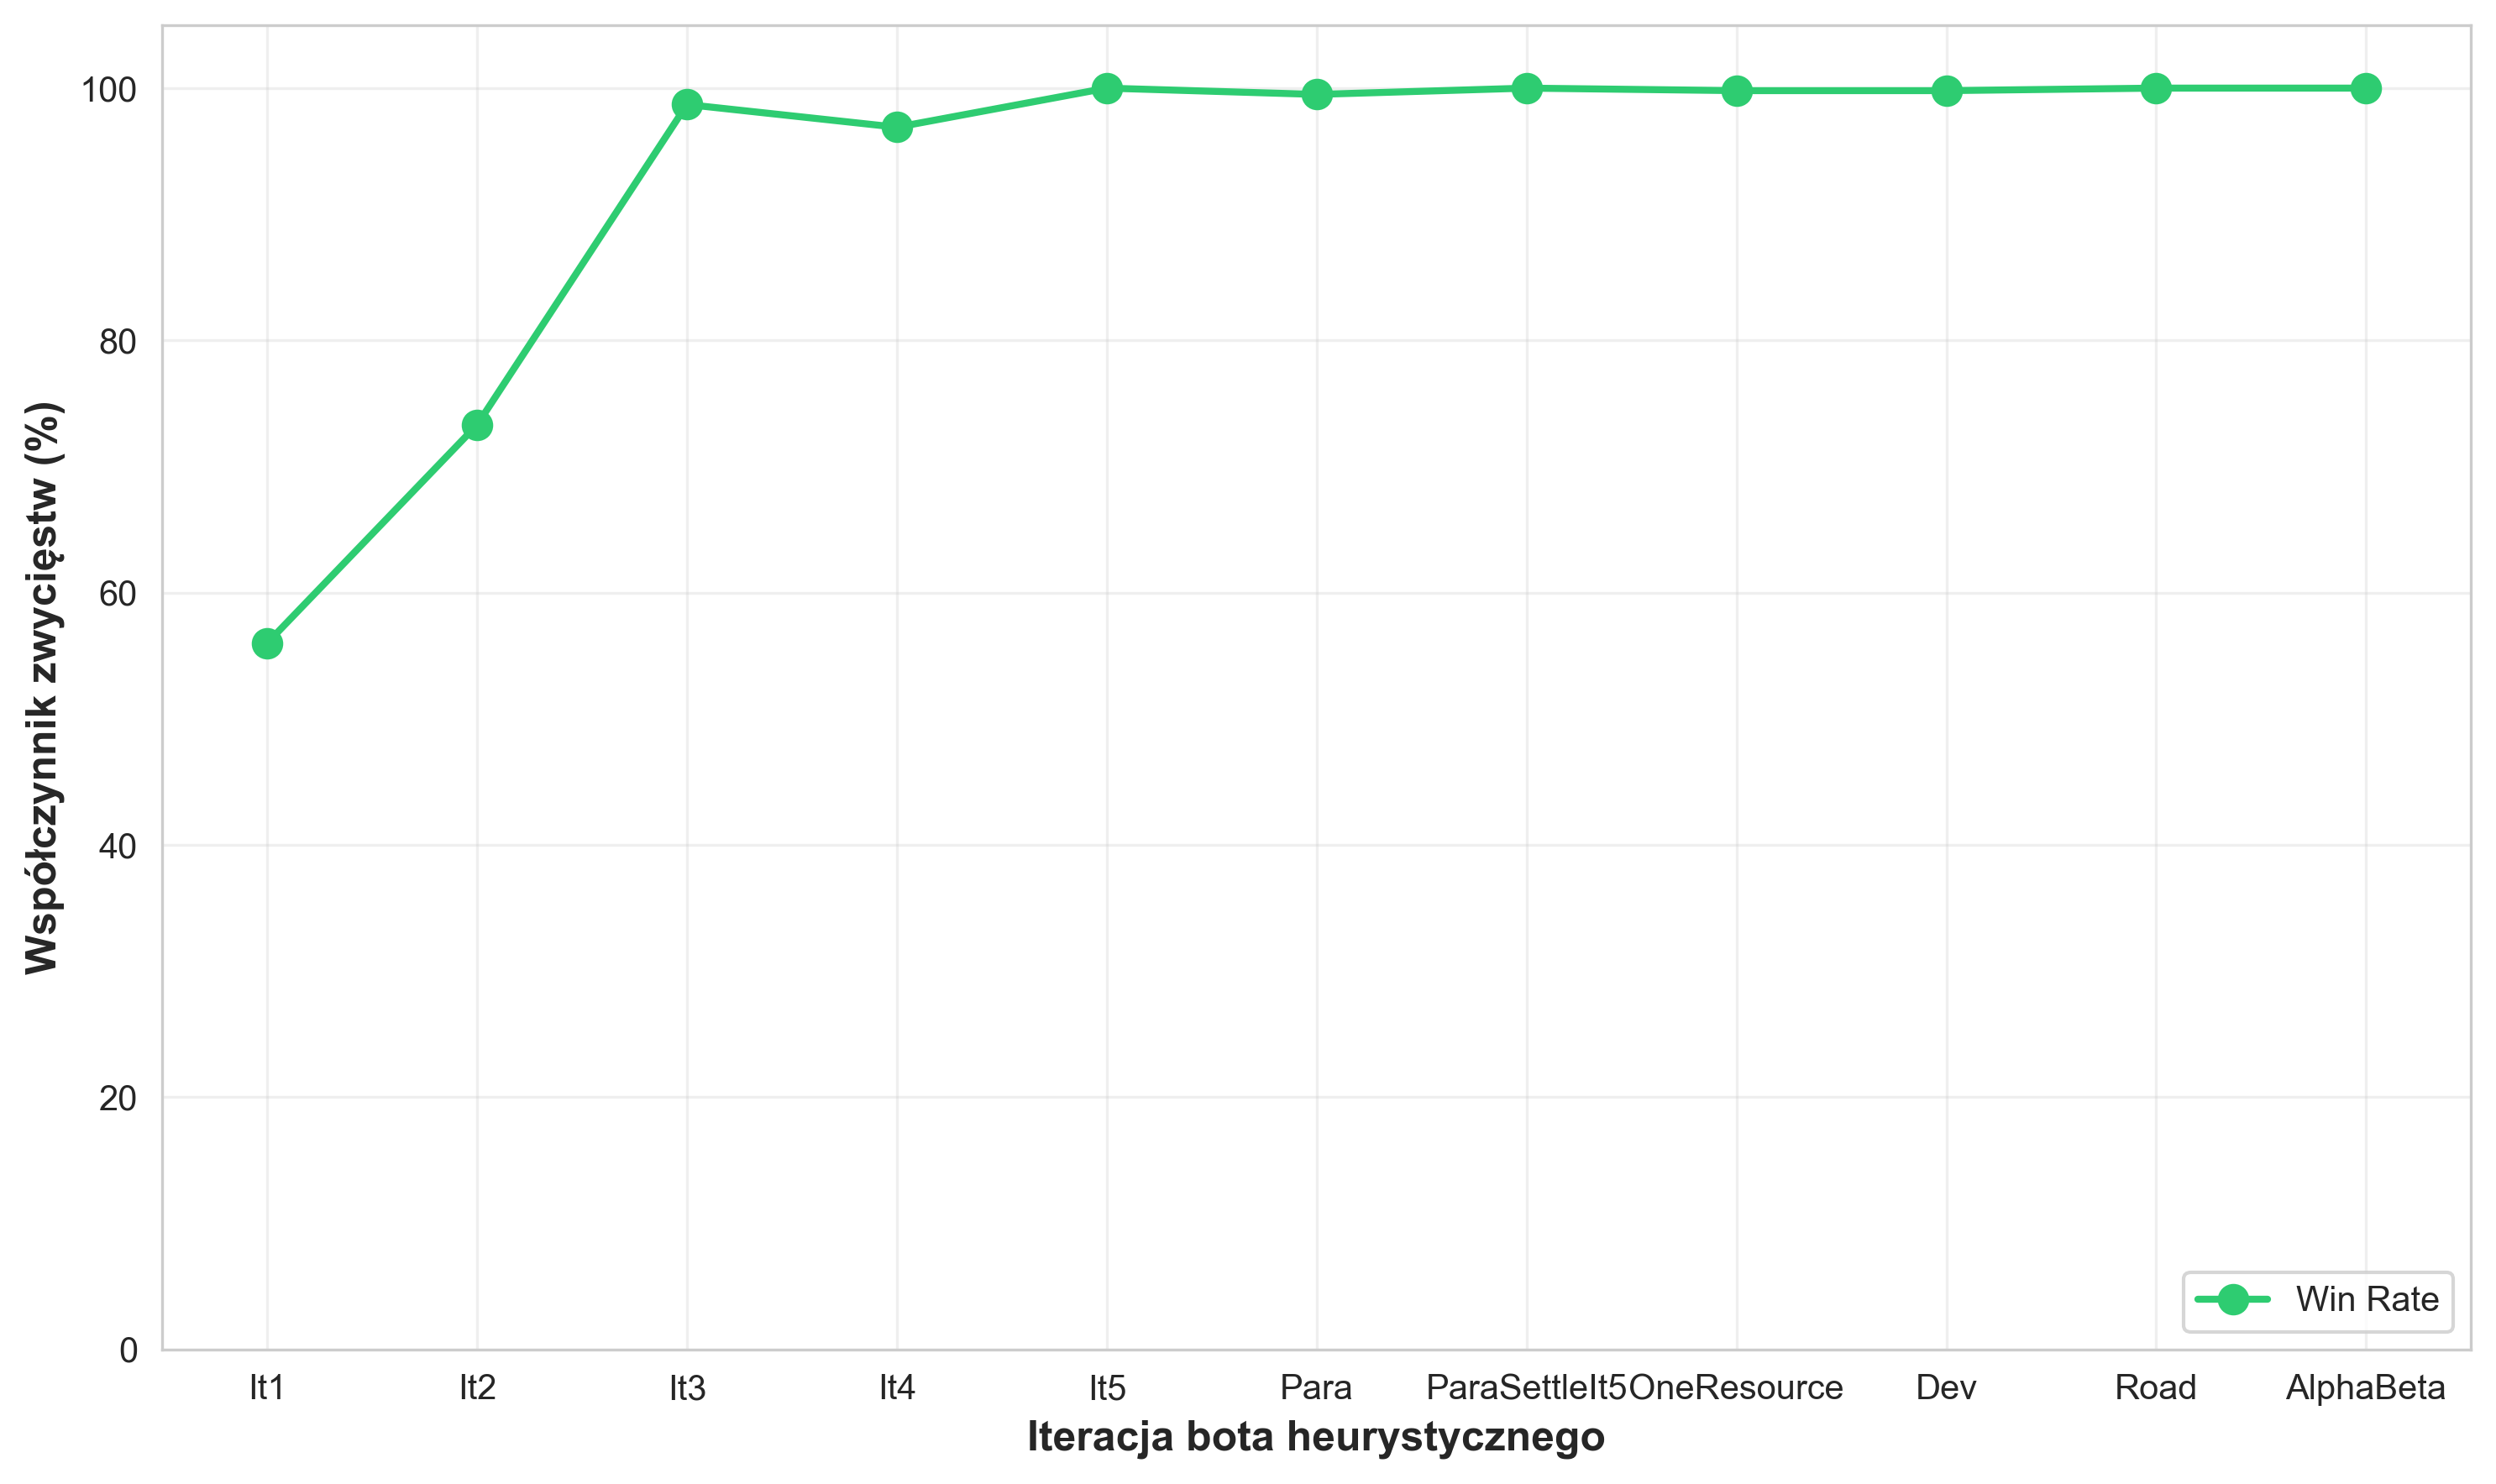
\includegraphics[width=0.8\textwidth]{rp_progression.png}
\caption{Zmiana wybranych metryk wraz ze wzrostem jakości botów}
\end{figure}

\textbf{Zależność tempa od jakości strategii}

Analiza średniej liczby tur pokazuje wyraźną korelację między jakością strategii a tempem rozgrywki. Wczesne iteracje botów (It1, It2) charakteryzują się bardzo długimi rozgrywkami --- odpowiednio 448.5 i 381.0 tur. Jest to konsekwencja niskiej skuteczności tych botów oraz braku zdolności do deterministycznego domykania partii, co prowadzi do przedłużających się rozgrywek, w których losowy przeciwnik ma realne szanse na zwycięstwo.

Przełom następuje wraz z wprowadzeniem It3, gdzie średnia liczba tur spada dramatycznie do 180.3, co stanowi redukcję o ponad 50\% w stosunku do It2. Ta zmiana jest bezpośrednio związana z jakościowym skokiem skuteczności --- bot przejmuje kontrolę nad rozgrywką i efektywnie kończy partie, nie pozwalając przeciwnikowi na przedłużanie rozgrywki.

Kolejne iteracje (It4, It5) oraz zaawansowane boty (Para, ParaSettleIt5, AlphaBeta) utrzymują szybkie tempo rozgrywki, osiągając średnią liczbę tur w zakresie 108--193. Szczególnie wyróżnia się AlphaBetaPlayer z najkrótszą średnią liczbą tur (108.7), co potwierdza, że algorytmy przeszukiwania drzewa gry są w stanie najszybciej identyfikować optymalne ścieżki prowadzące do zwycięstwa.

Warto zauważyć, że niektóre strategie wyspecjalizowane (OneResourcePlayer: 159.9 tur, DevPlayer: 166.1 tur) wykazują nieco wolniejsze tempo niż zaawansowane boty heurystyczne. Jest to związane z ich jednostronnym podejściem strategicznym, które może prowadzić do dłuższych rozgrywek, gdy specjalizacja nie jest wystarczająco efektywna.

\begin{figure}[h]
\centering
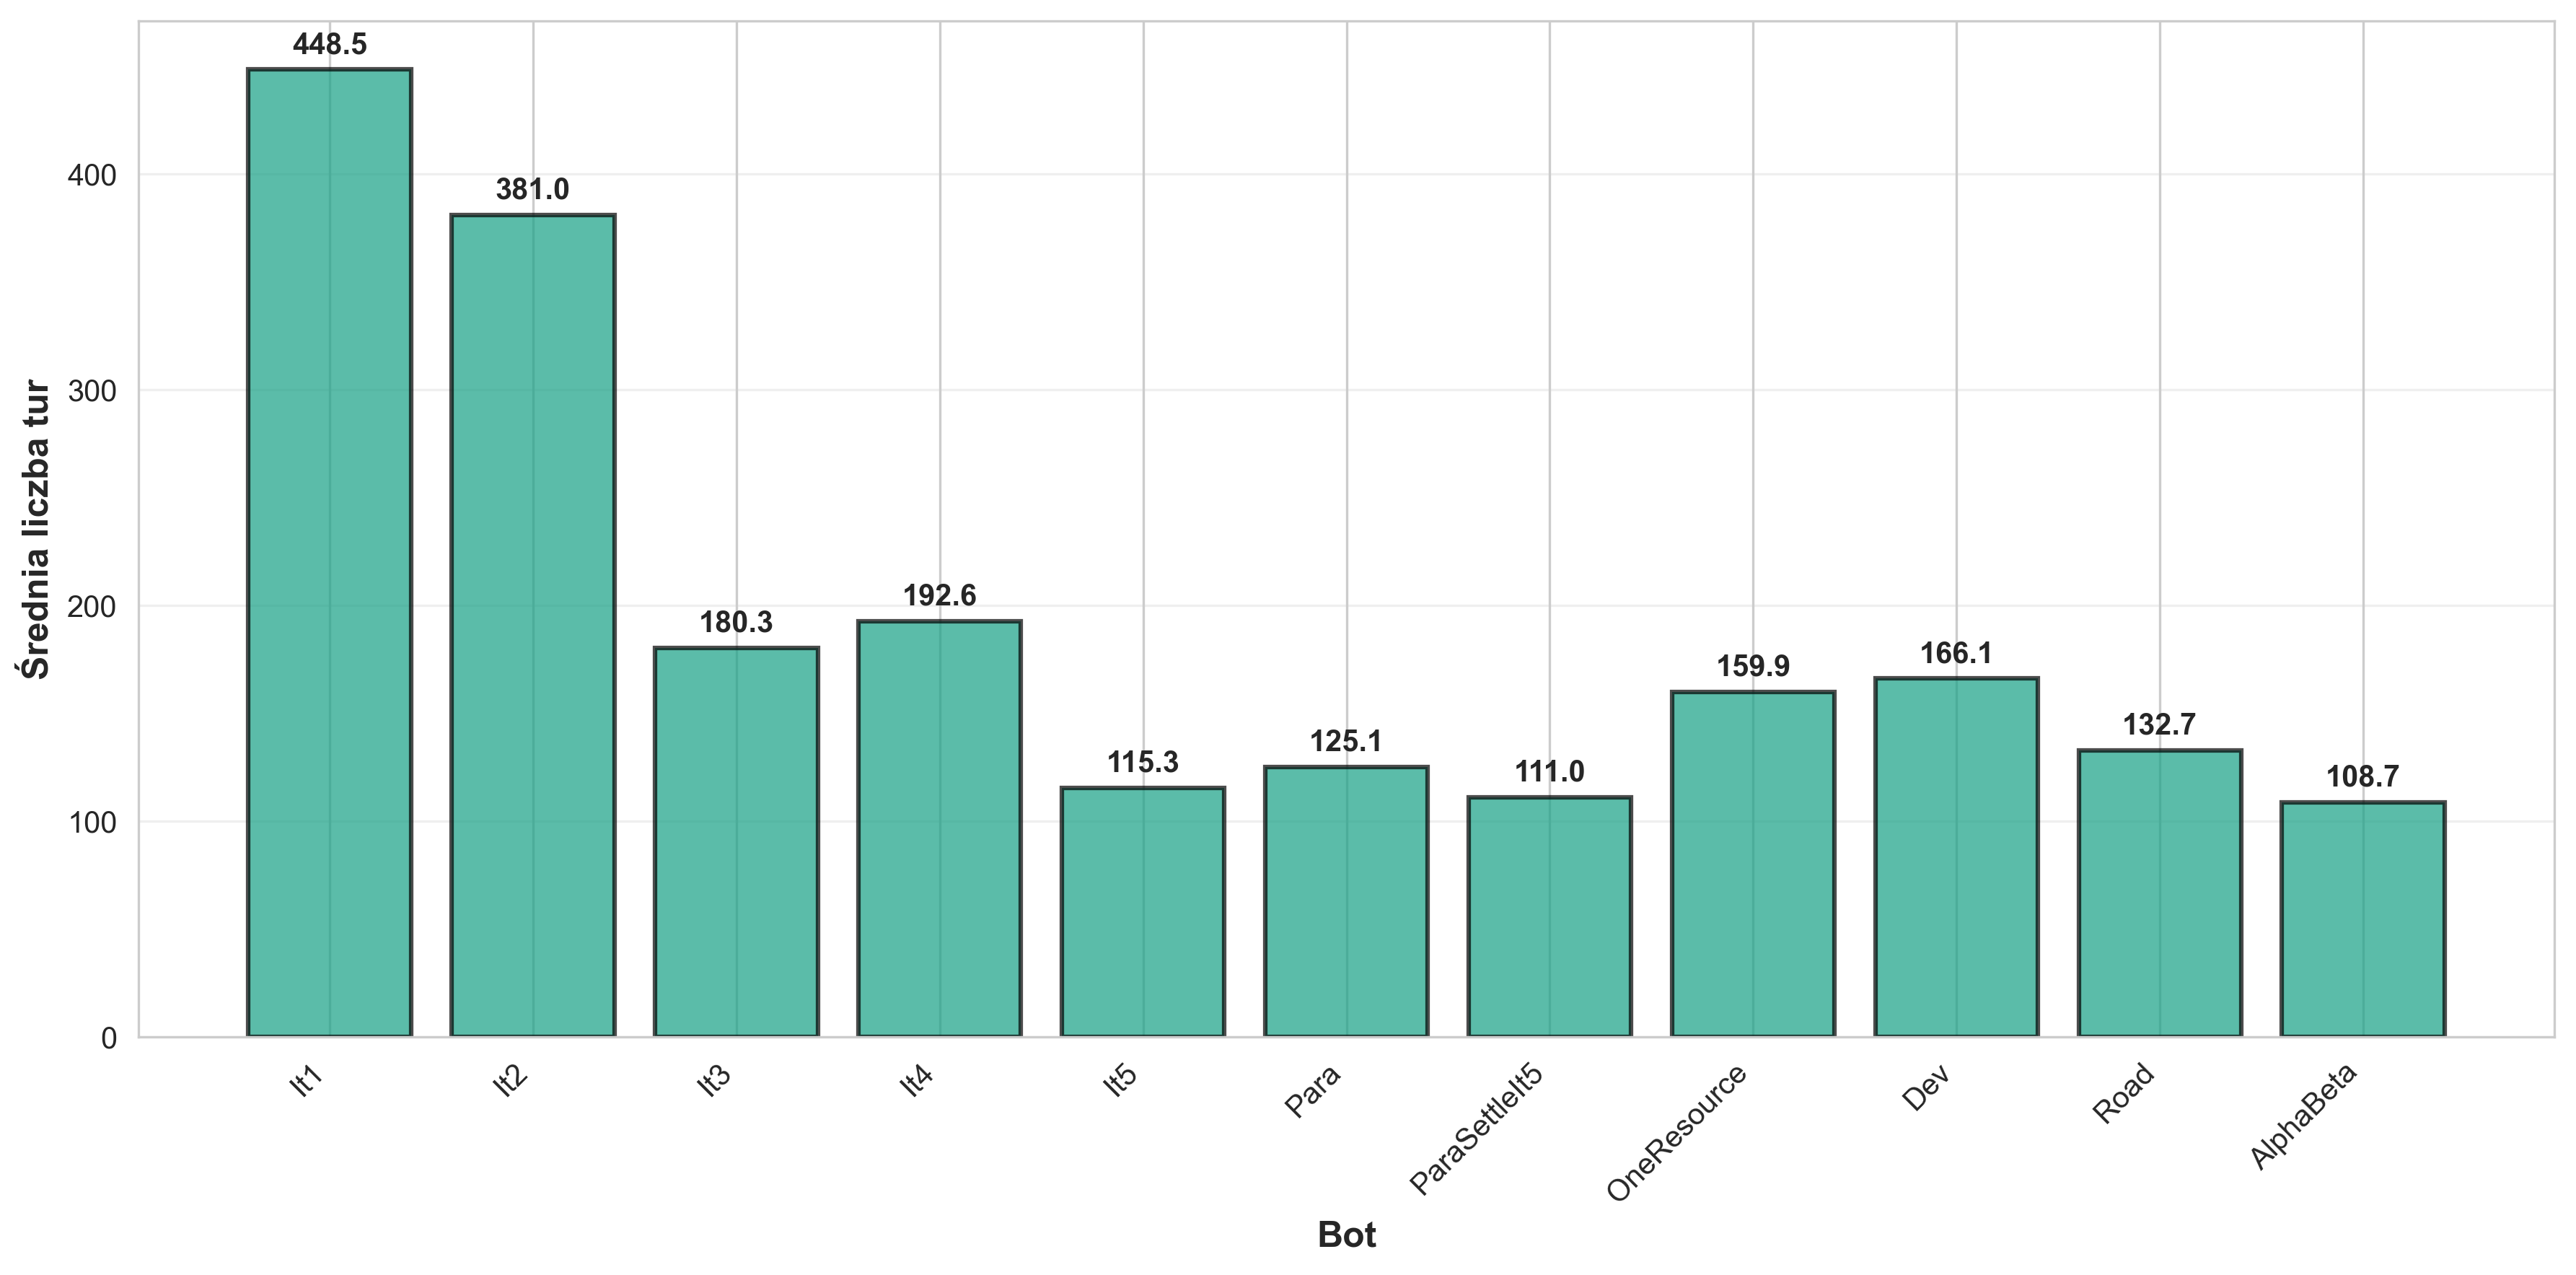
\includegraphics[width=0.8\textwidth]{rp_tempo.png}
\caption{Zależność tempa rozgrywki od jakości strategii}
\end{figure}

\textbf{Metryka LossVP}

Metryka LossVP (Bot) mierzy średnią liczbę punktów zwycięstwa przeciwnika w momencie, gdy bot przegrywa rozgrywkę. Wyższa wartość tej metryki oznacza, że bot przegrywa w późniejszych fazach gry, gdy przeciwnik zdążył już zgromadzić znaczącą liczbę punktów, co może wskazywać na bardziej wyrównaną rozgrywkę.

Analiza wyników pokazuje interesujący wzorzec: wczesne iteracje (It1, It2) przegrywają przy stosunkowo niskich wartościach VP przeciwnika (7.51 i 8.48), co sugeruje, że przegrywają one w różnych fazach rozgrywki, często wcześnie. Wraz z poprawą jakości botów, wartości LossVP (Bot) rosną --- It3 osiąga 11.50, a It4 9.80. To wskazuje, że bardziej zaawansowane boty przegrywają rzadziej, ale gdy już to robią, przeciwnik zdążył osiągnąć wyższy poziom rozwoju.

Szczególnie interesujące są wyniki dla strategii wyspecjalizowanych: DevPlayer osiąga najwyższą wartość LossVP (Bot) wynoszącą 12.00, podczas gdy OneResourcePlayer również osiąga 11.50. To sugeruje, że gdy te strategie przegrywają, dzieje się to w późniejszych fazach rozgrywki, gdy przeciwnik zdążył już rozwinąć swoją infrastrukturę.

\begin{figure}[h]
\centering
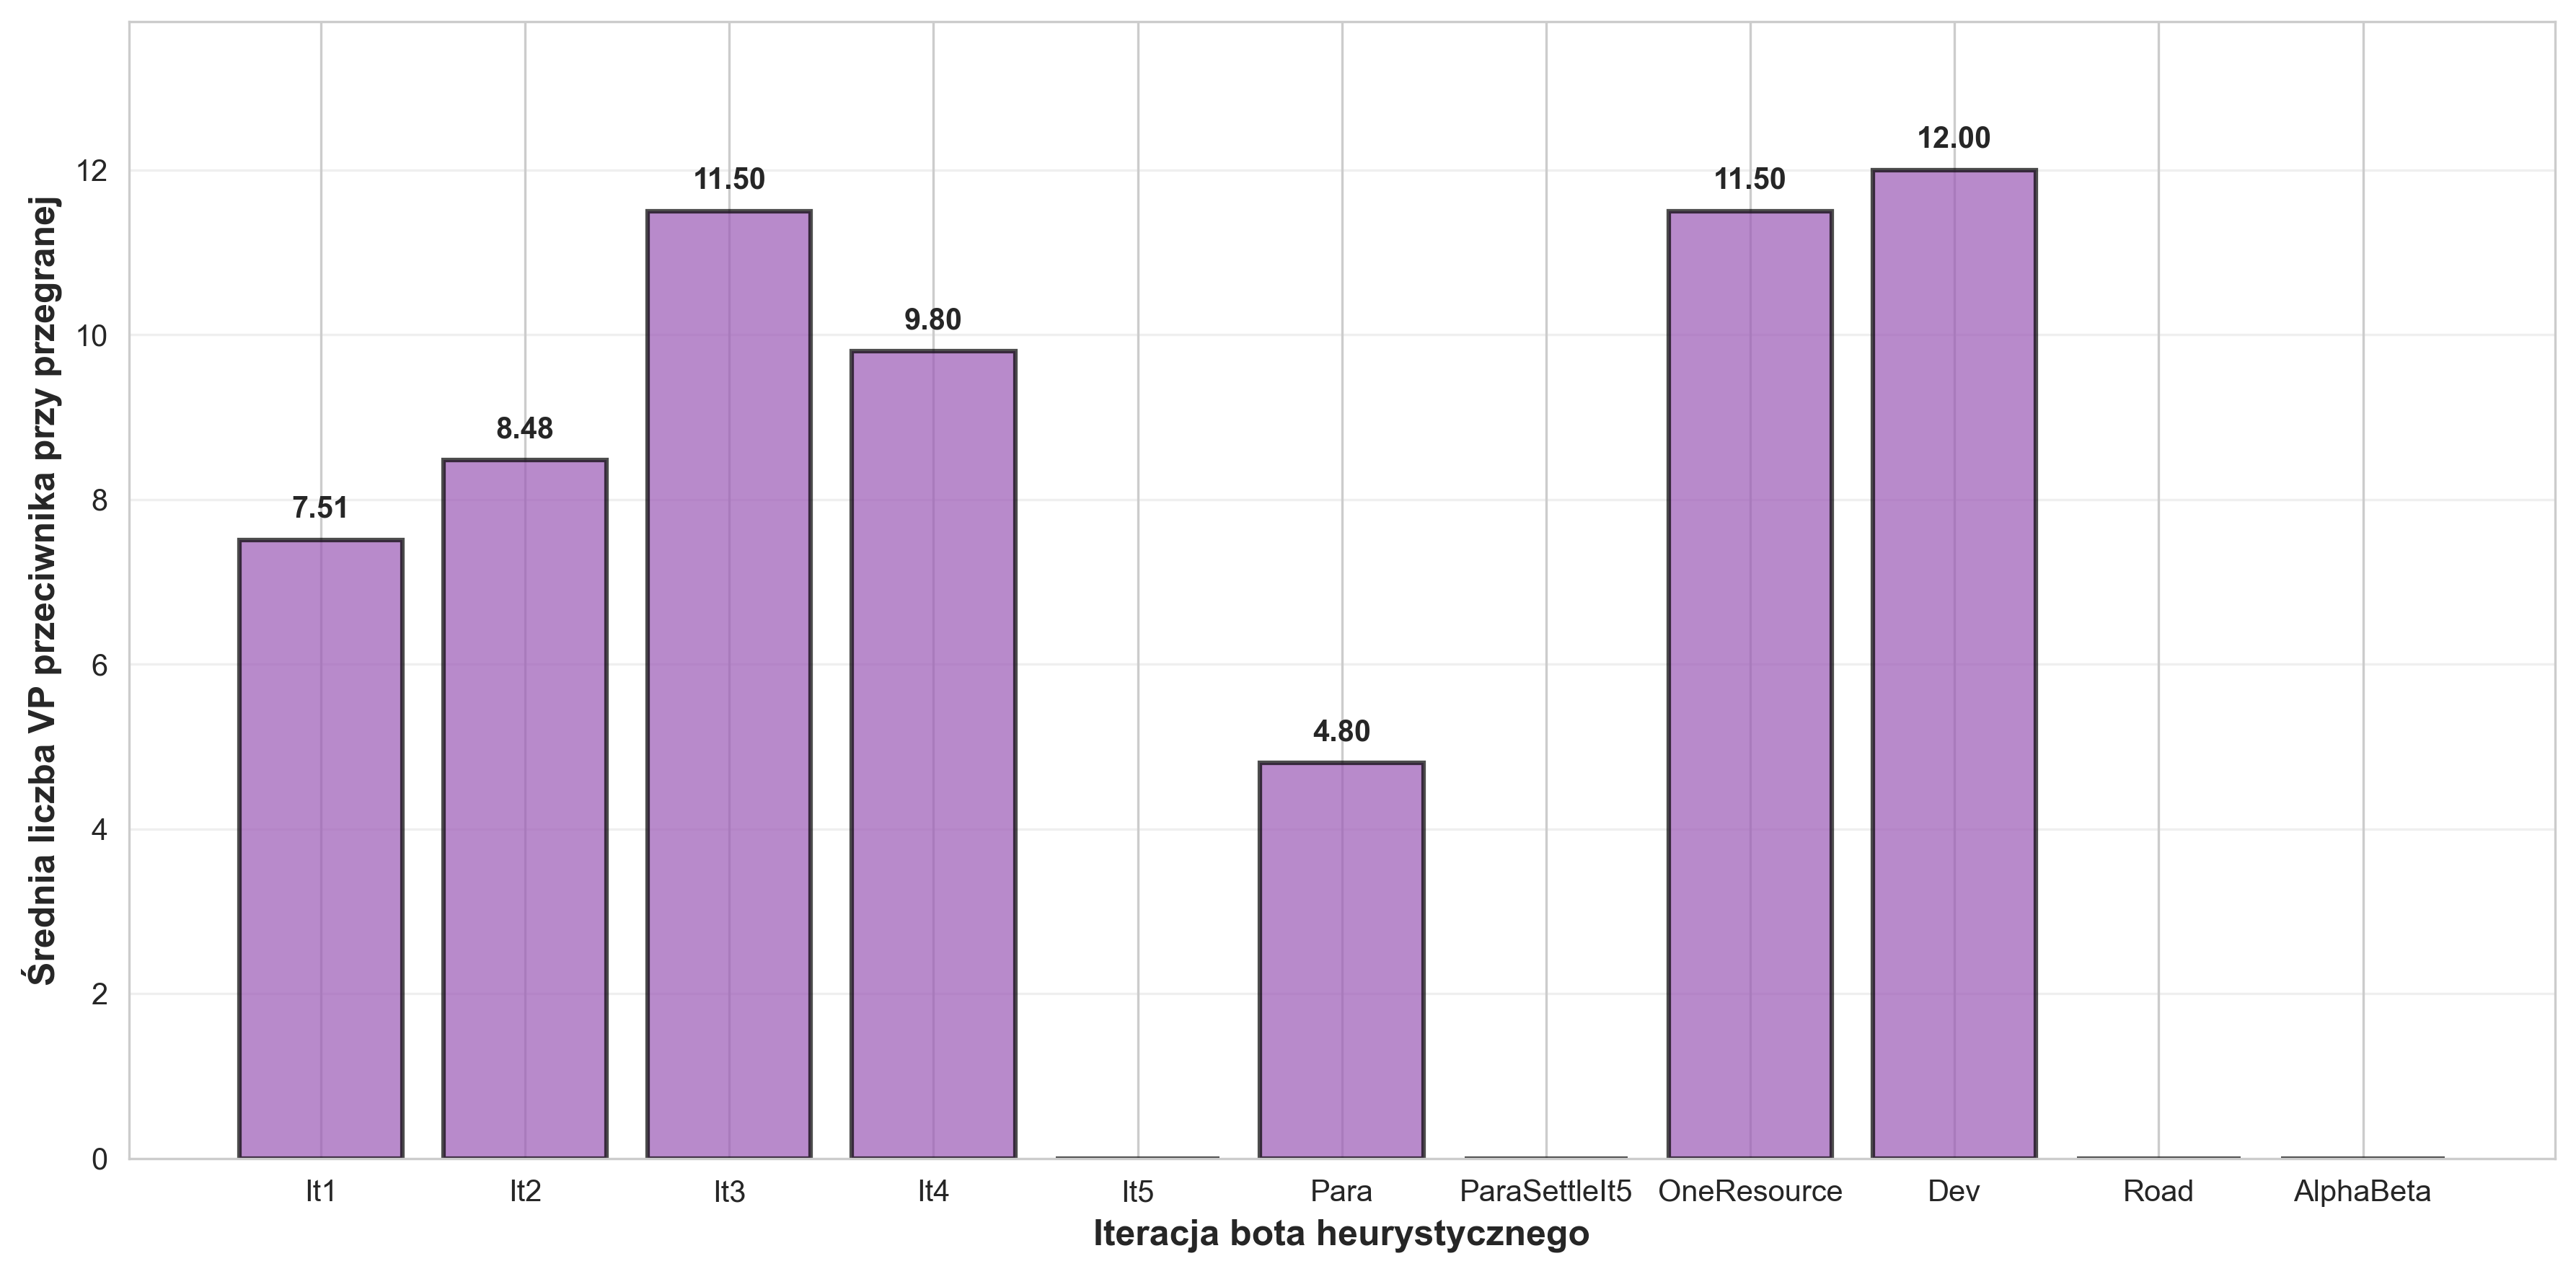
\includegraphics[width=0.8\textwidth]{rp_dominance.png}
\caption{Przewaga botów nad RandomPlayer --- średnia liczba VP przeciwnika przy przegranej}
\end{figure}

\textbf{Metryki dodatkowe}

Analiza dodatkowych metryk pozwala na głębsze zrozumienie charakterystyki strategii poszczególnych botów oraz mechanizmów ich działania.

\textbf{Premie strategiczne:} Współczynniki zdobycia premii \textit{Najdłuższa Droga} i \textit{Największa Armia} pokazują wyraźne różnice w podejściu strategicznym. Boty heurystyczne (It3--It5) osiągają wysokie wartości dla obu premii (71--95\% dla Najdłuższej Drogi, 87--99\% dla Największej Armii), co wskazuje na zbalansowane podejście. ParaPlayer wyróżnia się bardzo wysokim współczynnikiem Najdłuższej Drogi (90.2\%), ale niskim dla Największej Armii (25.9\%), co jest związane z jego strategią ekspansji terytorialnej kosztem kart rozwoju. DevPlayer pokazuje odwrotny wzorzec --- dominuje w Największej Armii (99.7\%), ale osiąga jedynie 52.8\% dla Najdłuższej Drogi, co odzwierciedla jego specjalizację w strategii kartowej.

\textbf{Karty rozwoju:} Średnia liczba zakupionych kart rozwoju waha się od 2.5 (AlphaBeta) do 9.9 (ParaPlayer). ParaPlayer wyróżnia się zdecydowanie najwyższą wartością, co jest konsekwencją jego strategii opartej na eksploracji różnych opcji decyzyjnych. Większość botów heurystycznych utrzymuje wartość w zakresie 2.9--3.7 kart na rozgrywkę, podczas gdy DevPlayer, zgodnie ze swoją specjalizacją, osiąga 4.6 kart.

\textbf{Produkcja zasobów:} Metryka ProdScore pokazuje wyraźną progresję wraz z poprawą jakości botów. It1 osiąga 730.4, podczas gdy It4 osiąga najwyższą wartość wśród botów heurystycznych (1190.3). ParaPlayer osiąga najwyższą wartość w całym zestawie (1267.8), co potwierdza skuteczność jego zbalansowanego podejścia strategicznego. AlphaBetaPlayer osiąga 1168.2, co jest wartością wyższą niż większość botów heurystycznych, co wskazuje na efektywne wykorzystanie zasobów przez algorytm przeszukiwania drzewa gry.

Wszystkie te metryki łącznie pokazują, że poprawa jakości botów przekłada się nie tylko na wyższy współczynnik zwycięstw, ale również na bardziej efektywne wykorzystanie mechanizmów strategicznych dostępnych w grze, co prowadzi do szybszych i bardziej deterministycznych rozgrywek.
